\thispagestyle{plain}
\section{Introduction}
\markboth{Introduction}{}


% Figures
% * Organoid technologies overview
% * Layered anatomy of organoid and primary
% * Single cell technologies overview
% * 


The human brain is a remarkably complex organ, made up of a vast diversity of cell types which are assembled into intricate structures. Understanding how its development is orchestrated has long been a central challenge in developmental biology. While studies in humans are challenging due to both ethical and practical reasons, we have already learned a lot about the molecular mechanisms that shape these processes by examining them in various non-human vertebrates.

During early embryogenesis, a sheet of neuroepithelial cells folds in and pinches off to form the neural tube, which gives rise to the central nervous system. Through a spatially and temporally precise cascade of morphogen gradients, the tube is segmented into distinct regions that will eventually develop into forebrain, midbrain, hindbrain and spinal cord. Each of these gradients is induced by a discrete group of adjacent cells, so-called organizers, which express and secret a defined set of morphogens. Most knowledge about this process has been gained from knockout and transplantation experiments in model organisms such as mice, with bulk genomic measurements or tissue stainings of a limited set of markers genes as a readout. As these conventional methods are limited in their throughput and resolution, it has long remained challenging to finely dissect differentiation events and underlying regulatory networks. Further, there are strong differences between the human and the mouse brain with respect to cellular composition, size, morphology and function, and it is unclear whether insights from mouse studies can be transferred to human brain development. Two emerging technologies are now transforming the field and offer exciting new possibilities to study human brain development at unprecedented resolution: ​\textit{In vitro} brain models grown from human stem cells ("brain organoids") and single-cell genomics.

% To "the" study might be suboptimal phrasing (Fatima), let's see
In this thesis, we want to harness and combine these new technologies to take a fresh approach to the study of human brain development. In particular, we are interested in shedding light on the regulatory landscape coordinates the diversification of brain regions in humans. For this, we first develop new computational tools that help us characterize regional identities in brain organoids (Chapter 2) and infer gene regulatory relationships from modern genomic measurements (Chapter 3). Next, we apply these tools (and others) to better understand gene regulatory mechanisms underlying brain development (Chapter 3 \& 5) and to interrogate regulatory origins of Autism Spectrum Disorder (Chapter 4). Before delving into these results, I will provide a primer on the technological advances that this work builds upon.

\clearpage


\subsection{Brain organoids}

Given the right culturing conditions, human stem cells can differentiate and self-organize into complex 3D tissues, so called organoids. Organoids can mimic the microanatomy and functionality of various organs, including the brain. The ability to grow such tissues in controlled culture environments has revolutionized the study of human biology and disease in recent years. This is especially true for the human brain, where primary tissue is hard to obtain and which is inaccessible to genetic manipulation. The following section should serve as an overview of current approaches to culture brain organoids and discuss strengths and limitations of organoids in modeling human brain development.


\subsubsection{Brain organoid technologies}

Brain organoid generation typically starts with aggregation of pluripotent stem cells into spheroids or embryoid bodies (EBs). EBs are then cultured in a neural induction medium, which pushes cells towards a neuroectodermal fate. After the neuroectoderm is established, the tissue further self-organizes to form lumens lined with neural progenitor cells, so-called neural rosettes. The emergence of this neuroepithelial stage can be aided by embedding in matrigel, a gel containing extracellular matrix components (\cite{lancaster_cerebral_2013,eiraku_self-organizing_2011}). Progenitor cells proliferate and can eventually differentiate into various neuronal and glial cell types that make up the mature organoid (Figure 1.1). Culturing in certain specialized media can further boost neuron differentiation and specification of neuronal subtypes (\cite{bardy_neuronal_2015}). 


Without the addition of external patterning factors, organoid development is not directed towards any brain-regional identity. Interestingly, organoids grown with such unguided protocols nevertheless contain cell populations resembling multiple distinct brain regions such as forebrain, midbrain or hindbrain (\cite{lancaster_cerebral_2013,kadoshima_self-organization_2013}). This offers the potential to study how different parts of the brain self-organize and interact during development. Understanding the molecular factors governing theses self-patterning mechanisms could be informative about the gene-regulatory basis of neurodevelopmental fate decisions in humans. However, there are disadvantages to this strategy: Regional composition can vary widely between different stem cell lines or even different batches from the same line (\cite{kanton_organoid_2019}) and predicting it \textit{a priori} is currently not possible. This can be particularly problematic if modeling a disease requires the generation of a specific brain region.

\begin{figure}[t!]
  \centering
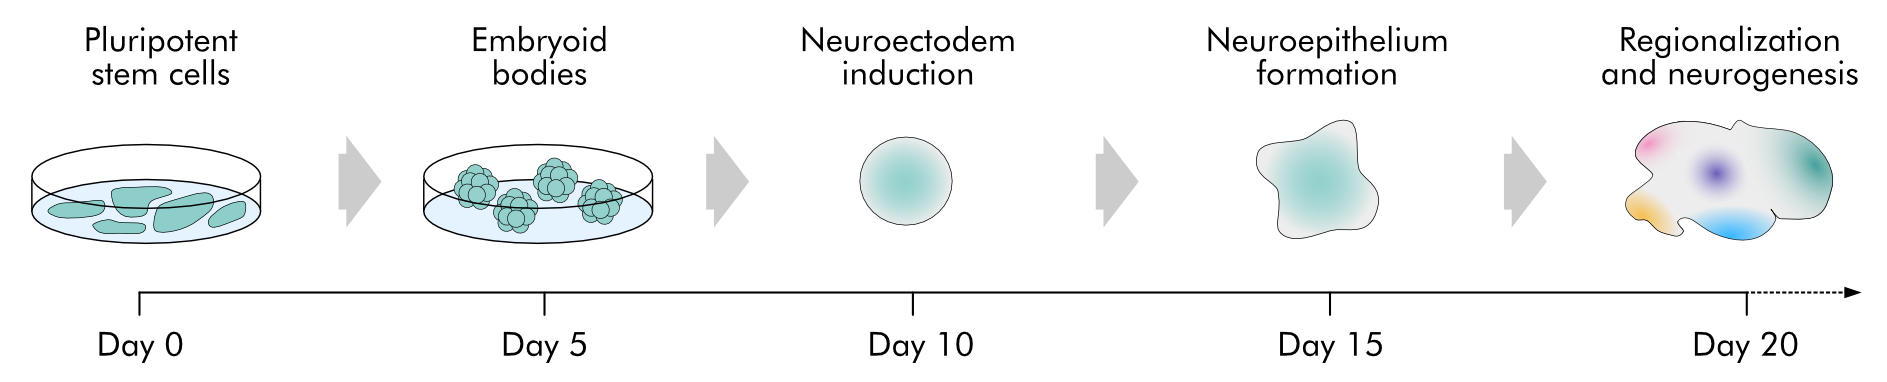
\includegraphics[width=\textwidth]{figures/introduction/Figure_organoid}
  \caption{\textbf{Making multi-region brain organoids from pluripotent stem cells.} First, pluripotent stem cells are aggregated into balls to form embryoid bodies. By culturing them in a specialized medium, neuroectoderm formation is induced, which later develops into a structured neuroepithelium. Later, neuroepithelial progenitor cells regionalize and give rise to neurons and other cell types in the mature organoid. The timeline shown here is based on the protocol developed by \cite{lancaster_cerebral_2013}.}
  \label{fig:intro3}
\end{figure}

An alternative strategy to grow brain organoids are guided protocols, which use signalling molecules to control patterning of the neuroepithelium to form a defined brain structure. These protocols take inspiration from  developmental biology and supply molecules interacting with known pattering pathways in the mammalian brain (reviewed in \cite{chiaradia_brain_2020}). For instance, WNTs and BMPs dorsalize the neural tube (\cite{dickinson_dorsalization_1995,saint-jeannet_regulation_1997}) and modulating these pathways has been successfully used in a number of studies to generate organoids resembling dorsal forebrain structures (\cite{xiang_fusion_2017,pasca_functional_2015,qian_brain-region-specific_2016,qian_sliced_2020}). Using this guiding paradigm, protocols have already been developed to generate various brain structures, including cortex (\cite{eiraku_self-organizing_2011,kadoshima_self-organization_2013,pasca_functional_2015,velasco_individual_2019}), ventral forebrain (\cite{miura_generation_2020,birey_assembly_2017,xiang_fusion_2017,bagley_fused_2017}), hypothalamus (\cite{qian_brain-region-specific_2016}), thalamus (\cite{xiang_hesc-derived_2019}), midbrain (\cite{qian_brain-region-specific_2016,monzel_derivation_2017,kim_modeling_2019}) and others. 

% Fatima: MISTR not organoids, "multiple brain structures [in a single organoid]"
Furthermore, there are approaches to expose the tissue to a spatial gradient of one or a combination of morphogens to control the induction of multiple brain structures within the same tissue (\cite{rifes_modeling_2020,cederquist_specification_2019}). This can also be achieved by fusing organoids resembling one or more brain structures into so-called assembloids (\cite{bagley_fused_2017,birey_assembly_2017,xiang_fusion_2017}, reviewed in \cite{pasca_rise_2018}), which can be very useful for studying neuronal migration and formation of inter-region neuronal connections. This set of guided protocols might enable reproducible generation of brain structures and modeling region-specific diseases.



\subsubsection{Organoids model brain development \textit{in vitro}}

Brain organoids have been shown to recapitulate certain aspects of human brain development, such as characteristic microanatomy and cell type diversity. Even without the addition of external patterning factors, they can give rise to organizer-like populations (\cite{renner_self-organized_2017}), and eventually form distinct brain region identities. The tissue morphology of these brain regions can be very similar to their primary counterpart: Like in the fetal human cortex, the neural rosettes of the organoid neuroepithelium begin to develop a layered architecture along an apical-basal axis (\cite{kadoshima_self-organization_2013,lancaster_cerebral_2013}). Apical (or ventricular) radial glia (RG) cells line the apical ventricular zone (VZ) and differentiate into intermediate progenitor cells (IPs), occupying the sub-ventricular zone (SVZ). IPs further differentiate into neurons, which migrate along basal extended processes of RGs to populate the basally located cortical plate. Younger organoids primarily give rise to deep layer-like neurons, but after around 4 months of culture in optimized conditions, more diverse neuronal populations can emerge and stratify into deep and upper layers (\cite{kanton_organoid_2019,qian_sliced_2020}). However, some aspects of this tissue architecture are to date still lacking in organoids. For instance, the fetal cortex has a distinct layer of RG cells in the outer SVZ, so-called outer or basal radial glia cells (oRG/bRG). While oRG marker genes are expressed in some organoid cells, they lack the distinct spatial separation of this layer (\cite{bhaduri_cell_2020}). Optimizing oxygenation and nutrient diffusion as well as longer culturing times could be beneficial for more reliable development of cortical layers in organoids (\cite{bhaduri_cell_2020,chiaradia_brain_2020}).

Generally speaking, cell types arising in organoids resemble primary counterparts to a remarkable degree (\cite{camp_human_2015}). Both unguided and guided protocols can give rise to glutamatergic (excitatory) and GABAergic (inhibitory) neurons with transcriptomic signatures resembling various distinct brain structures. As outlined above, dorsal forebrain-derived excitatory neurons can resemble different cortical layers (\cite{kanton_organoid_2019,qian_sliced_2020}), but they can be also derived from other brain structures, such as diencephalon, midbrain or hindbrain (\cite{kanton_organoid_2019}). 
% Remove because of Fatimas edit: "For instance, Cajal-Rezius cells, a class of diencephalon-derived excitatory neurons, have been identified in multiple guided and unguided organoid protocols (\cite{kanton_organoid_2019,velasco_individual_2019})"
Inhibitory neurons in the primary human cortex are born in the ganglionic eminences (GEs) located in the ventral forebrain and migrate into the cortex during development. Such GE-derived inhibitory neurons can also be found in organoids, both in unguided protocols (\cite{kanton_organoid_2019}) and guided protocols patterned for forebrain or specifically ventral forebrain (\cite{velasco_individual_2019,birey_assembly_2017,miura_generation_2020}). In some cases, they even possess distinct regional transcriptomic signatures of lateral-, medial- or caudal GE (\cite{kanton_organoid_2019,miura_generation_2020}). 

A wave of neurogenesis during early brain development is preceded by gliogenesis, where various glial cell types are produced that are crucial for brain function (\cite{rowitch_developmental_2010}). This is recapitulated in organoids, where glial cell types also arise after sufficiently long culturing times. Astrocytes, which perform many functions in the brain, can be very abundant in brain organoids and even overgrow neurons in very long cultures ($\geq$ 4 months) (\cite{kanton_organoid_2019,giandomenico_cerebral_2019,sloan_human_2017}). Moreover, oligodendrocytes and oligodendrocyte progenitors, which go on to create the myelin sheath around neuronal axons, can develop in organoids (\cite{tanaka_synthetic_2020}). Their induction can also be specifically induced through alterations in the protocol (\cite{madhavan_induction_2018,marton_differentiation_2019}). Such protocols are promising, as they might help to better control proportions of certain cell types to better mimic primary tissue.

Despite fast progress in the development of new and refined organoid protocols, there also remain several limitations to brain organoids as model systems. Because all brain organoids to date are derived exclusively from the neuroectodermal lineage, they are inherently missing cells from other germ layers, most importantly mesoderm, which gives rise to microglia and endothelial cells of blood vessels. Microglia are tissue-resident immune cells that infiltrate the brain early in development and later play a role in synaptic pruning (\cite{favuzzi_gaba-receptive_2021,paolicelli_synaptic_2011}). As a result of lacking vascularization, nutrient and oxygen supply is limited by diffusion, which becomes increasingly insufficient if the organoids grow larger. This leads to a necrotic core especially in older organoids and limited maturation of neurons as mentioned above (\cite{vertesy_cellular_2022,bhaduri_cell_2020}). To overcome those limitations, some recent protocols specifically induce the generation of such cell types in organoids (\cite{cakir_engineering_2019,cakir_expression_2022}).

Moreover, the lack of stereotypic patterning often results in high variability between orga-noids grown from different stem cell lines or in separate batches. While the transcriptomic signatures of cell types are generally reproducible, the proportion of different cell types can vary drastically, especially with unguided protocols (\cite{kanton_organoid_2019}). Furthermore, there is so far no comprehensive reference of organoid cell types, which makes it often challenging to interpret and annotate data from new organoid protocols. Thus, increasing the reproducibility of organoid culture and developing robust methods for rapid phenotyping are crucial especially for larger-scale drug screening applications. 



\subsubsection{Applications of brain organoids}
Given the many parallels between human fetal and organoid brain development as well as the human genomic context, it is not surprising that human brain organoids have quickly emerged as useful model systems. In particular, organoids allow us to address biological questions that cannot be studied in humans directly and for which mice and other model organisms are not appropriate models. Brain organoids can also readily be genetically and chemically manipulated and even grown from patient cell lines, which gives them unprecedented advantages over animal models. 

Disease modeling is currently one of the most prominent applications of brain organoid technology. Especially brain malformations are well suited to be studied in organoids, due to their early onset and strong disease phenotypes (\cite{klaus_altered_2019,lancaster_cerebral_2013}). More recently, autism spectrum disorder (ASD) has also been studied in organoids by introducing haploinsufficiency for three ASD risk genes (\cite{paulsen_autism_2022}). Furthermore, organoids have successfully been used to model infectious diseases affecting the brain, such as the Zika virus (\cite{qian_brain-region-specific_2016,dang_zika_2016}) and to screen for antiviral compounds (\cite{zhou_high-content_2017}). 

Organoids also offer fresh opportunities to study the genetic mechanisms underlying brain evolution. By growing organoids from cell lines of primates such as chimpanzee and macaque and comparing them with human organoids, studies have explored evolutionary differences in brain developmental timing and identified human-specific gene expression patterns and regulatory regions (\cite{kanton_organoid_2019,mora-bermudez_differences_2016,pollen_establishing_2019}).

These results demonstrate that organoid systems offer great potential as model systems of the human brain and the combination with genome editing techniques and chemical screening makes them especially powerful to study mechanisms of human brain development in health and disease.


\subsection{Single-cell genomics}

% First paragraph good, but then too much on atlases. Should probably be more of an aside in the context of the thesis
% - Atlases help to phenotype
% - Instead, focus on development -> multiome -> GRN -> perturbation
% - Then lead into the following sections
% - Better motivation with context to the thesis topic

During development from pluripotency, organoids turn from relatively homogenous balls of stem cells into complex tissues with many cell types and diverse regional identities. Studying organoid development and resolving differentiation events thus requires probing them on the level of individual cells. Over the past decade, an exciting new set of tools has emerged to perform increasingly information-rich measurements of various phenotypic features in single cells. Initial methods focused on gene expression by bringing RNA-sequencing to the single-cell regime (\cite{tang_mrna-seq_2009,islam_characterization_2011}). Since then, the repertoire of single-cell technologies has expanded to allow measurements of various genomic readouts as well as proteins and spatial features. The throughput of these assays has also scaled up rapidly (\cite{svensson_exponential_2018}) and modern commercial solutions now allow profiling up to 1 million individual cells in a single experiment (\cite{srivatsan_massively_2020,mulqueen_high-content_2021}). 

Advances in measurement technologies are accompanied by the development of computational methods to deal with increasingly large and complex datasets (\cite{zappia_exploring_2018}). Next to tools developed specifically for single-cell genomics, many methods for high-dimensional data analysis from other areas of statistics and machine learning have proven very useful in the single-cell genomics realm. Such modern analytical tools have become essential components of data analysis workflows to perform pre-processing, quality control and sophisticated data analyses and interpretation. The combination of high-throughput and high information content assays with advanced computational methods now allows us to take a systems-level view at biology and have already significantly advanced our understanding of biological systems.

% Possibly expand on this
These technological advances are also critical for studying developmental processes in organoids for three main reasons:

\begin{enumerate}
    \item {\scshape Primary references}: The power to characterize molecularly distinct cell types in complex tissues without prior purification has catalyzed many studies surveying composition of primary human and mouse brain tissue (\cite{la_manno_molecular_2021,zeisel_molecular_2018,polioudakis_single-cell_2019,mayer_developmental_2018}). These brain cell atlases are valuable references for understanding organoid development and cell type identities.
    \item {\scshape Developmental trajectories}: Analyzing tissues at single-cell resolution allows us to capture all intermediate cell states between precursors and differentiated cells in a single snapshot. This can reveal continuous changes in gene expression that occur along the differentiation path and help identify intermediate cell states. 
    \item {\scshape Regulatory inference}: Integrating single-cell transcriptomic and epigenomic measurements opens up new opportunities for inferring gene regulatory relationships. Additionally, genetic perturbation screens with single-cell genomic readout can further elucidate causal relationships between gene regulation and phenotype.
  \end{enumerate}

In the following sections, I will describe how different genomic modalities can be measured on a single-cell level and outline how we can combine these modalities to better understand gene regulation. Finally, I will discuss how perturbation experiments can help reveal causal relationships and how they can be employed in a high-throuput manner with single-cell readout.


\subsubsection{Single-cell transcriptomics}

In order for (protein coding) genes to exert their function on the cell, they first need to be transcribed into mRNA, spliced, translated into an amino acid sequence and folded into functional proteins. These molecular machines then perform most functions in a cell. Regulating the transcription of genes is one way for a cell to control which proteins are active at any given time. Different cell types express distinct subsets of genes, which lets them perform specialized functions. Measuring genome-wide mRNA transcript abundance of a cell (collectively called the \textit{transcriptome}) using single-cell RNA-sequencing (scRNA-seq) has thus become a useful way to characterize cell types. 

\begin{figure}[H]
  \centering
  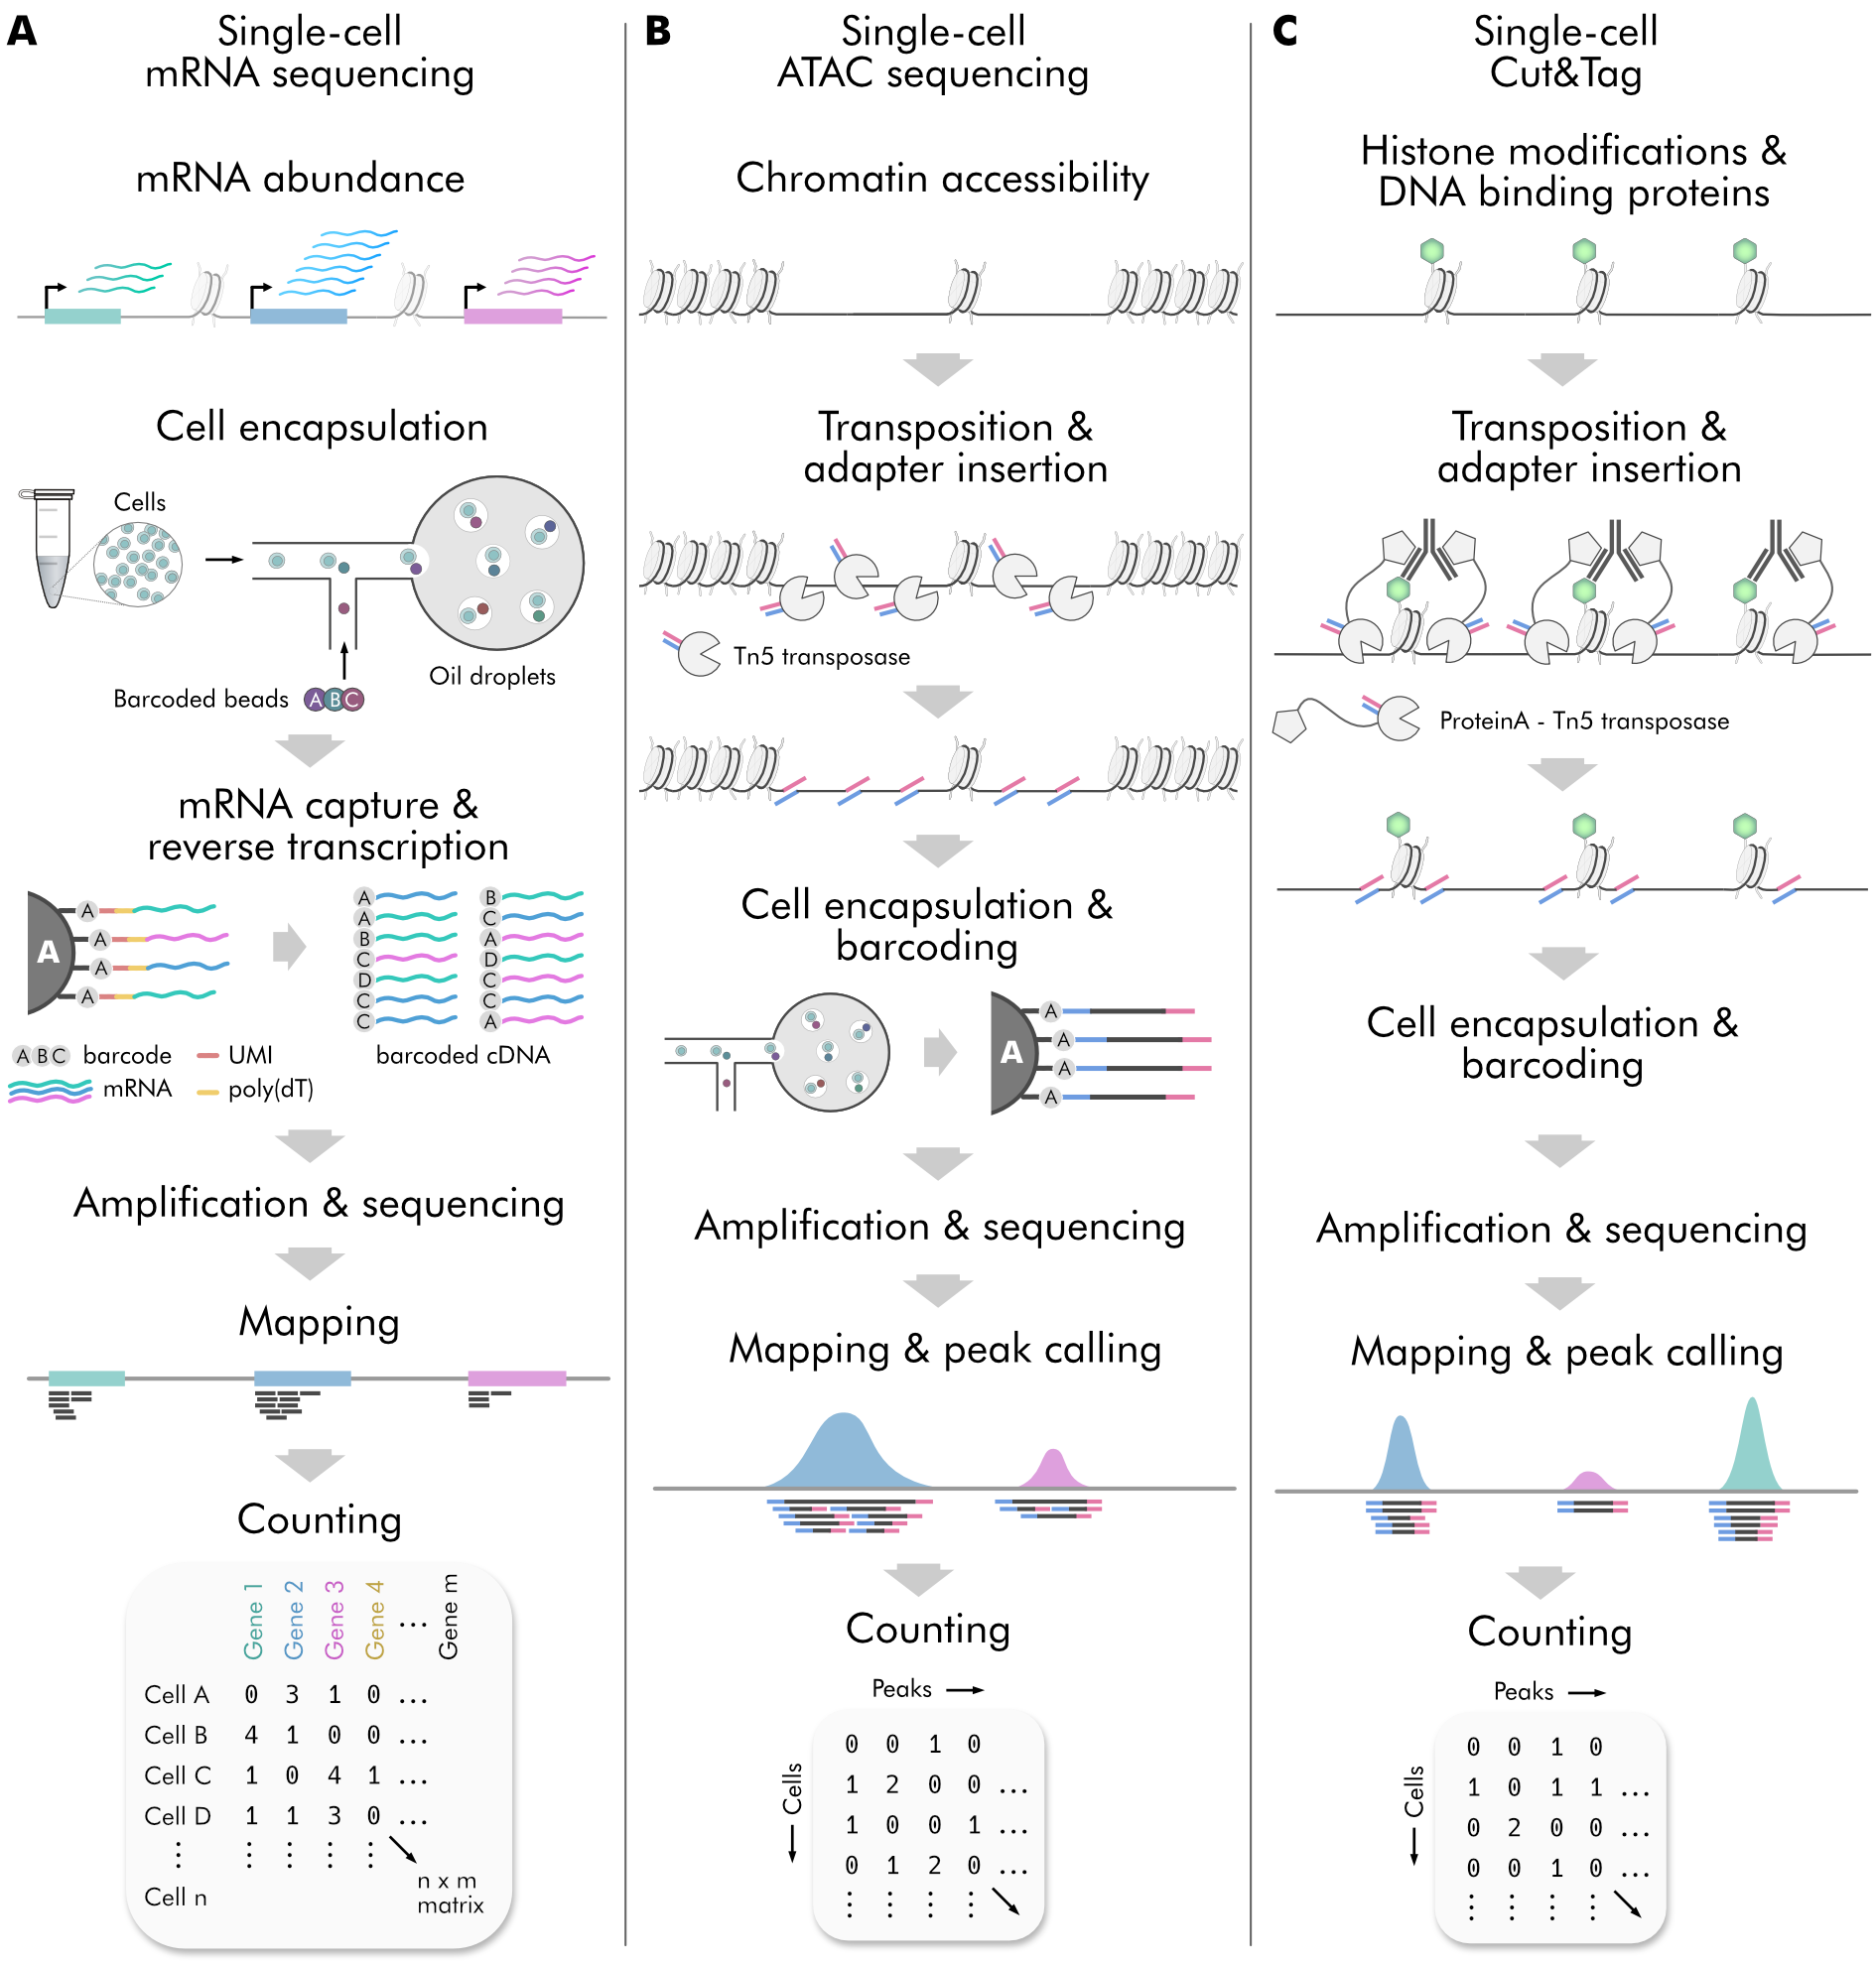
\includegraphics[width=\textwidth]{figures/introduction/Figure_tech}
  \caption{\textbf{Single-cell genomic technologies used in this thesis.} 
  Schematic overview of single-cell sequencing methods based on the 10X genomics chromium platform. (A) Single-cell mRNA sequencing (scRNA-seq) measures transcriptome-wide mRNA transcript abundance. First, the tissue is dissociated into single cells, which are then encapsulated with barcoded beads and enzymes into oil droplets on a micofluidic chip. Poly-A tails of mRNAs are captured on the barcoded beads, where they are reverse transcribed to obtain barcoded cDNA libraries. Libraries are then amplified and sequenced using next-generation sequencing methods. The resulting sequencing reads are mapped to a reference. Counting of UMIs and demultiplexing cell barcodes yields a cell-by-transcript count matrix. (B) Single-cell ATAC sequencing (scATAC-seq) measures genome-wide chromatin accessibility. Using a genetically engineered DNA transposase (Tn5), open chromatin regions are cleaved and adapter sequences are inserted. The resulting fragments are then conjugated to cell barcodes using a similar strategy as for scRNA-seq. After amplification and sequencing, fragments are mapped back to the genome to identify peaks marking accessible genomic regions. Demultiplexing cell barcodes and counting fragments per peak yields a cell-by-peak matrix. (C) Single-cell Cut\&Tag can be used to measure genome-wide occurrences of histone modifications or DNA binding proteins. A ProteinA - Tn5 fusion construct is specifically tethered to antibodies binding chromatin proteins and modifications. Cleavage and adapter insertion are therefore constricted to genomic sites near targeted proteins. All other steps are analogous to scATAC-seq.}
  \label{fig:intro2}
\end{figure}

ScRNA-seq is currently the most mature and most widely used method for single-cell molecular profiling. While there are many protocols and technologies for performing scRNA-seq, they all have some underlying principles in common. Individual cells are first lysed or permeabilized, then their mRNA molecules are reverse transcribed into complementary DNA (cDNA), provided with a unique cell barcode and amplified, often using polymerase chain reaction (PCR). Most modern protocols also add a unique molecular identifier (UMI; \cite{islam_quantitative_2014}) for each mRNA molecule in order to correct for amplification bias. The amplified cDNA library is further sequenced and finally a cell-by-transcript count matrix is obtained by aligning sequencing reads to a transcriptome reference and assigning reads to individual cells based on the cell barcode. ScRNA-seq protocols predominantly differ in how unique cell barcodes are introduced. Most of the earliest methods that were developed isolate individual cells into (micro-)wells or microfluidic chambers, where they are lysed and supplied with individual barcodes (e.g. \cite{picelli_smart-seq2_2013,shalek_single-cell_2014,jaitin_massively_2014,treutlein_reconstructing_2014}). Some of these methods are highly sensitive with respect to transcriptome coverage, but they are limited in the number of cells they can profile in a single experiment. More recent droplet-based methods, such as Drop-seq (\cite{macosko_highly_2015}), inDrops (\cite{klein_droplet_2015}) or the commercial 10x Genomics Chromium platform (\cite{zheng_massively_2017}), use microfluidic chips to encapsulate cells in oil droplets containing barcoded beads. These methods allow profiling thousands of cells in parallel and are currently most widely used in the field (Figure 1.2A). To achieve even higher throughput, recent methods rely on a split-pool-barcoding paradigm and can scale to millions of cells (\cite{rosenberg_single-cell_2018,yin_high-throughput_2019,cao_comprehensive_2017}). Here, the cells are never physically isolated, but a unique combinatorial index is introduced by iterative barcode ligation, pooling and splitting. These compounding technological developments have lead to an exponential increase in throughput of cells over the past decade (\cite{svensson_exponential_2018}).

All of these methods can ultimately yield a cell-by-transcript count matrix, which is the basis for most downstream analysis (Figure 1.3). Initially, it is commonly normalized to correct for count depth bias arising from sampling effects. Normalizing scRNA-seq data is an active topic of research (\cite{lause_analytic_2021,hafemeister_normalization_2019,townes_feature_2019,vallejos_normalizing_2017}), but the most widely used method is log-normalization:

\[ x^{\prime}_{ij} = log(\lambda \cdot  \frac{x_{ij}}{\sum_{j}{x_{ij}}} + 1)  \]

Here, counts $x$ for each transcript $j$ in each cell $i$ are divided by the total counts for this cell, multiplied by a constant scaling factor $\lambda$ (usually $10^4$ or $10^6$) and subsequently log-transformed with a pseudocount of 1. After normalization, the high dimensionality of the expression matrix can be reduced with dimensionality reduction algorithms like principal component analysis (PCA). The goal is to capture most of the variance in as few dimensions as possible, as this reduces the computational burden, removes noise and can be advantageous for distance calculations. Leading principal components (PCs) of the expression matrix are therefore used as the input for many downstream tasks, such as clustering, visualization or inference of differentiation trajectories (Figure 1.3). There are best-practice recommendations for various subsequent analysis steps (\cite{luecken_current_2019}), however they can vary depending on the biological question at hand.

\begin{figure}[t!]
  \centering
  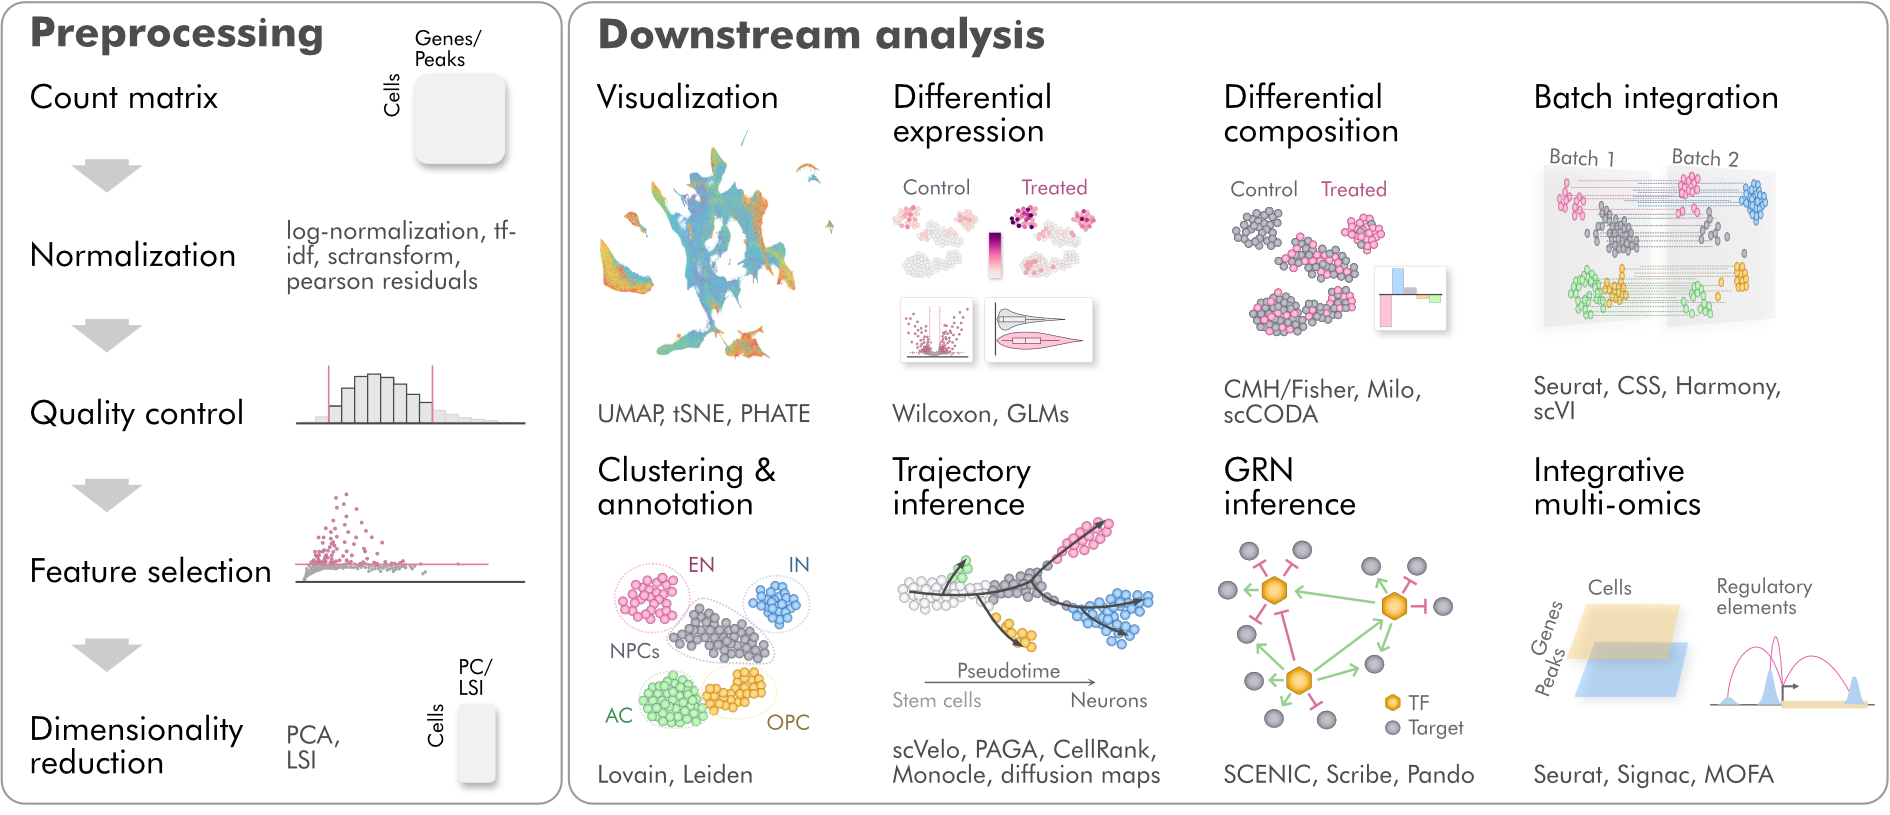
\includegraphics[width=\textwidth]{figures/introduction/Figure_comp}
  \caption{\textbf{Overview of computational analysis steps for single-cell genomics data.} 
  Typical preprocessing steps and downstream analysis tasks indicating examples of commonly used tools and algorithms. After generating the count matrix, preporcessing involves a number of common steps. Normalization aims to remove sequencing depth bias, quality control is done to remove low-quality cells and features selection aims to select the most informative features. After this, linear dimension reduction is usually performed using PCA or LSI. After these preprocessing steps, the analysis steps vary based on the biological question and experiemntal setup. Common tasks include visualizing the data in 2D, testing for differential expression or differential composition between conditions, integration of different batches, clustering of cells and annotation of cell types and states, inference of differentiation trajectories, gene regulatory network inference and integrative analyses between multiple omics layers. Reference for the tools and methods highlighted here can be found in Table S1.1}
  \label{fig:intro2}
\end{figure}

\subsubsection{Single-cell epigenomics}

All cells in complex tissues like organoids typically share the same genomic sequence, but adopt a variety of cell types by activating different sets of genes. We have seen above how the immediate \textit{result} of gene regulation, the transcriptome, can be read out using scRNA-seq. However, to understand cell differentiation and identity, we are also interested \textit{how} gene expression is regulated. These mechanisms, which allow the cell to differentially activate parts of the genome, are collectively referred to as the \textit{epigenome}. Emerging experimental methods can profile various aspects of the epigenome, including chromatin accessibility (\cite{buenrostro_single-cell_2015,cusanovich_multiplex_2015}), chromatin conformation (\cite{ramani_massively_2017,stevens_3d_2017}), DNA methylation (\cite{smallwood_single-cell_2014}) and histone tail modifications (\cite{kaya-okur_cuttag_2019,bartosovic_single-cell_2021,ku_single-cell_2019,hainer_profiling_2019}) in single cells. Here, we will focus on chromatin accessibility measurements using single-cell assay for transposase-accessible chromatin sequencing (scATAC-seq; \cite{buenrostro_single-cell_2015}) and profiling of histone marks using single-cell cleavage under targets and tagmentation (scCut\&Tag; \cite{kaya-okur_cuttag_2019}).

\begin{figure}[b!]
  \centering
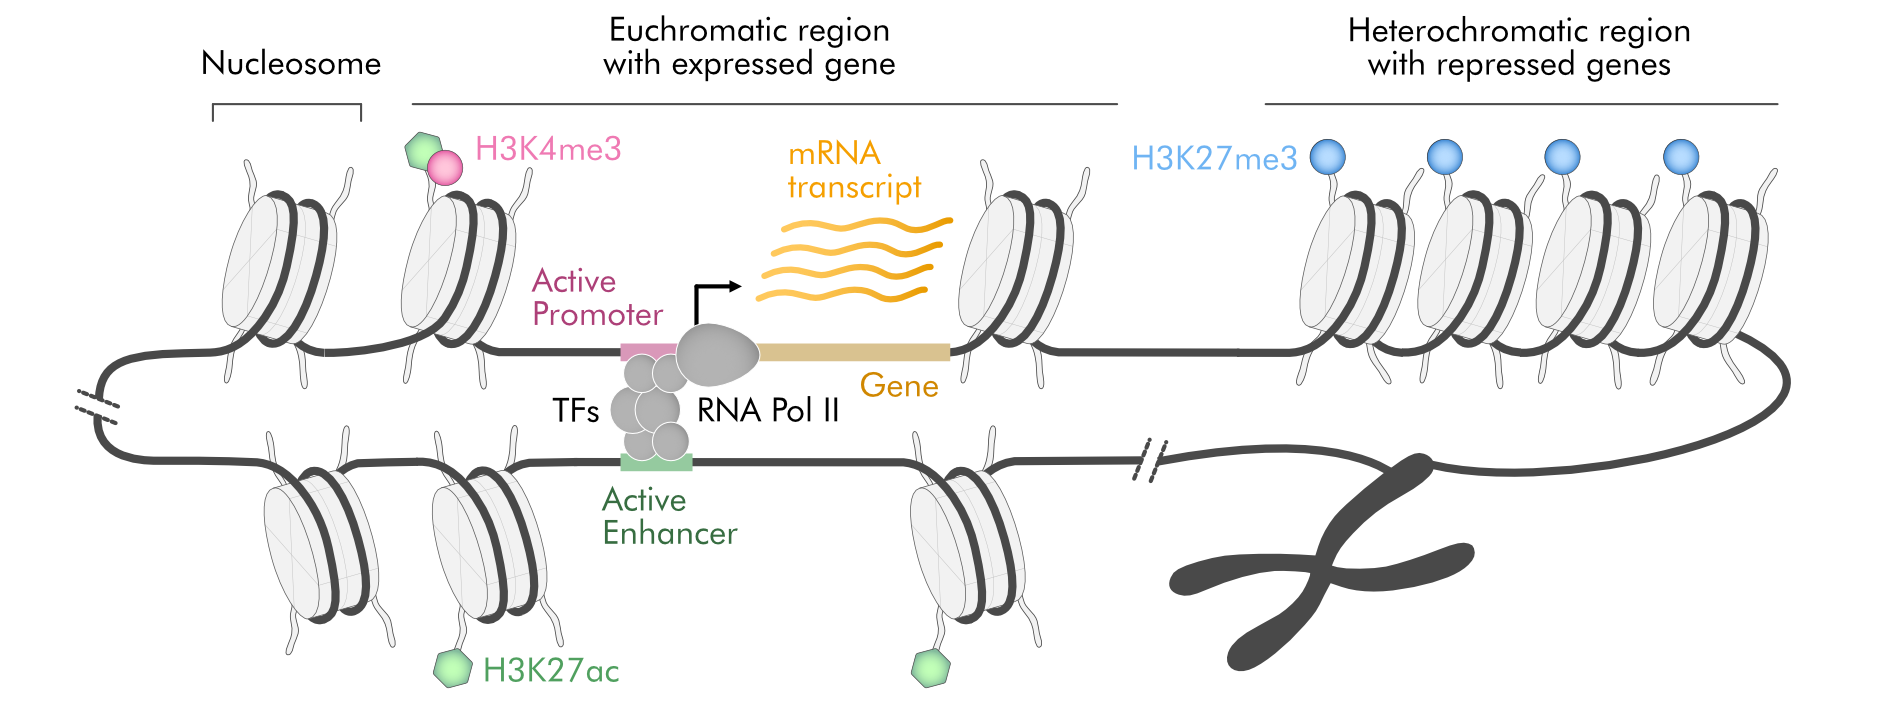
\includegraphics[width=\textwidth]{figures/introduction/Figure_chromatin}
  \caption{\textbf{Epigenetic mechanisms of gene regulation.} Loosely packed euchromatic regions allow transcription factors (TFs) to bind to \textit{cis}-regulatory elements, which facilitates the expression of genes. Promoters are regulatory elements close to the transcription start site and are marked by co-enrichment of the H3K27ac and H3K4me3 chromatin modifications. Enhancers are distal elements brought into proximity of the promoter through looping of chromatin, they are marked by H3K27ac. Heterochromatin is tightly packed, which does not allow genes to be expressed. These repressed regions are marked by H3K27me3.}
  \label{fig:intro3}
\end{figure}

Chromatin, the complex of DNA and associated proteins such as histones, can come in various levels of physical compaction. In its highly compacted form ("heterochromatin"), the DNA is tightly packed into an array of nucleosomes and generally enzymatically inaccessible (Figure 1.3). Some regions of the genome are opened by pioneer factors and more loosely packed as a result ("euchromatin"), which allows them to interact with other transcription factors (TFs) and the transcriptional machinery. As a result, chromatin accessibility is a hallmark of transcriptionally active genes as well as non-coding regions of DNA harboring TF binding sites ("\textit{cis}-regulatory elements"), such as active promoters and enhancers. ScATAC-seq can be used to obtain genome-wide accessibility profiles and is thus a valuable tool for understanding gene regulation (Figure 1.2B). The assay takes direct advantage of the fact that only open chromatin regions are enzymatically accessible to a genetically engineered hyperactive DNA transposase (Tn5), which cleaves open chromatin and inserts adapter sequences. Using similar techniques as for scRNA-seq, the resulting fragments can be conjugated to cell barcodes, amplified and sequenced. By mapping sequencing reads back to the genome, we can identify "peaks" marking accessible stretches of DNA (\cite{duan_model-based_2019}). After demultiplexing cell barcodes, we obtain a cell-by-peak matrix, which most downstream analyses are based on.

While chromatin accessibility broadly stratifies the genome into active and inactive regions, certain chemical modifications of histones can serve as even more precise markers of chromatin states. Post-translational modification of histone tails by acetyltransferases and methyltransferases can exert drastic effects on gene expression (Figure 1.3). For instance, acetylation of lysine 27 on histone 3 (H3K27ac) at enhancers and promoters coincides with activation of gene expression, while tri-methylation of the same residue (H3K27me3) has a repressive effect and generally marks heterochromatin (\cite{allis_molecular_2016}). Such histone modifications as well as other proteins interacting with the genome can be profiled genome-wide using scCut\&Tag (\cite{bartosovic_single-cell_2021,kaya-okur_cuttag_2019}). The experimental procedure of scCut\&Tag can be seen as an extension of scATAC-seq in which a ProteinA/Tn5 fusion construct (pA-Tn5) is specifically tethered to antibodies binding chromatin proteins and modifications (Figure 1.2C). Hence, transposition will be constricted to genomic sites near those targeted proteins. Analogous to scATAC-seq, peaks can be called from sequencing data of fragments to map locations of histone modifications and protein binding sites.

Peak matrices from both scATAC-seq and scCut\&Tag are very sparse (the majority of peaks is not detected in a given cell) and often thought of as effectively binary (a peak is either present/accessible or absent/inaccessible). Thus, many methods for normalization and dimensionality reduction were adopted from text mining, where a collection of documents is represented by sparse vectors of word occurrences. An example for this is the commonly used normalization method term frequency–inverse document frequency (tf-idf), which is intended to reflect how important a peak (word) is in a given cell (document) by emphasizing the contribution of highly variable peaks. Here, the relative frequency of peak $j$ in cell $i$ ("term frequency") is multiplied by the inverse frequency of the peak across all cells ("inverse document frequency") and then log-transformed:

\[ x^{\prime}_{ij} = log(tf_{ij} \cdot idf_{ij} + 1) \]

with

\[ tf_{ij} = \frac{x_{ij}} {\sum_{j}{x_{ij}}} \]

and 

\[ idf_{ij} = \frac{N}{\sum_{i}{x_{ij} > 0}} \]

where $N$ is the total number of cells and $\sum_{i}{x_{ij} > 0}$ the number of cells in which peak $i$ is non-zero. On a tf-idf matrix, dimensionality reduction can be performed via singular value decomposition (SVD). Performing SVD on a tf-idf matrix is also referred to as latent semantic indexing (LSI) and the leading LSI components are used for many downstream analyses which require a dimensionality-reduced feature space (\cite{stuart_comprehensive_2019}). From this point onward, the analysis of scATAC and scCut\&Tag datasets follows similar principles as for scRNA-seq data. However, integrating transcriptomic and epigenomic layers of information facilitates new types of analyses that are not possible with each individual modality alone.



\subsubsection{Integrative single-cell multi-omics}

Single-cell readouts from multiple genomics layers ("multi-omics") can be invaluable for understanding gene regulation, especially if they are matched for a given cell or population of cells. This can either be achieved if both modalities are integrated into a shared feature space or if they are measured simultaneously in the same cell. The latter is becoming more and more accessible with modern assays (\cite{ma_chromatin_2020,bartosovic_multimodal_2022}) and commercial solutions (10x Genomics multiome ATAC + Gene expression). Still, there remains a need to integrate existing datasets from individual modalities.

Integration typically requires all datasets to share a common feature space. Natively, this is not the case for scRNA-seq and chromatin data, which measure transcripts and genomic peaks, respectively. To facilitate integration, chromatin data can be used to compute "activity scores" for each gene by considering fragment counts on and around the gene body. Activity scores from assays marking active chromatin states are assumed to correlate positively with gene expression, and can therefore be matched with scRNA-seq data using common integration methods (\cite{stuart_comprehensive_2019,luecken_benchmarking_2022}). 

If multiple modalities are integrated or measured simultaneously, they can be correlated with each other to elucidate various features of gene regulation. For instance, peak accessibility can be correlated with gene expression to annotate distal elements regulating the transcription of the gene (\cite{ma_chromatin_2020}). Similarly, matching TF binding motifs in peak regions and correlating their accessibility with TF expression can refine TF binding site predictions. Matching two chromatin modalities can also yield valuable information such as active promoters marked by co-enrichment of histone marks H3K4me3 and H3K27ac. Taken together, these integrative analyses can reveal relationships between gene expression and chromatin states, which serves as a basis for inferring regulatory networks.



\subsubsection{Inference of gene regulatory networks}

Developmental cell state transitions are controlled by networks of transcription factors which control gene expression by binding to \textit{cis}-regulatory elements (CREs). CREs can be promoters close to the transcription start site (TSS) of a gene or distal enhancers that are brought into spatial proximity of the promoter by looping of chromatin. TFs binding to enhancers and promoters can recruit chromatin remodellers and the transcriptional machinery to regulate expression of the target gene. Transcribed genes are translated into protein and if they themselves are TFs, they can regulate the expression of other genes, forming a gene regulatory network (GRNs). Many features of this process can now be measured on the level of individual cells, which enables inference of genome-wide GRNs.

Most algorithms for GRN inference from transcriptomics data are based on the idea that TF expression should, to some degree, be correlated with the expression of the genes it regulates. In its most basic form, this results in a coexpression network inferred by computing correlation (\cite{stuart_gene-coexpression_2003}) or partial correlation (\cite{kim_ppcor_2015}) between TFs and target genes. More modern implementations use regression models to fit the expression of target genes as a function of TF expression (\cite{aibar_scenic_2017}). However, directionality of TF-TF interactions cannot be derived from coexpression alone. The incorporation of time course information or pseudo-temporal orderings can help with this, assuming there is a time-lag between regulator and target expression (\cite{qiu_inferring_2020}). Moreover, TF binding motif information can be used to constrain TF targets to genes with a predicted binding site in its vincinity (\cite{aibar_scenic_2017}). By integrating multi-omic single-cell data, we can go even further and leverage covariance relationships between chromatin states of regulatory regions and genes in addition to coexpression. This may facilitate inference of gene regulatory interactions at unprecedented resolution and scale.


\subsubsection{Perturbing gene regulation}
% General principles of perturbations
% * isogenic KO 
% * chemical perturbation
% * single-cell mosaic KO
% Mosaic KO approaches
% Applications 
% Challenges

GRN inference from genomics data is a useful strategy to generate hypotheses about gene regulation, but causal inference solely from observational data is difficult. Moreover, even if the full GRN is known, it is currently not sufficient to predictively model cell behavior like state transitions or bifurcations (\cite{teschendorff_statistical_2021}). Perturbation of regulatory networks using genetic knockouts or chemical treatment is therefore crucial to reveal causal relationships between regulatory features and complex phenotypes.

Perturbation experiments can either be performed in an arrayed fashion, where each sample (e.g. organoid) is perturbed and assayed separately, or pooled, where many perturbations are multiplexed in each sample. Arrayed perturbations such as isogenic knockouts or chemical treatments have the advantage that non-autonomous cellular phenotypes can be assessed on the level of entire tissues. Moreover, one usually has greater control over experimental variables as well as the choice of positive and negative controls. However, pooled genetic screens are more efficient and scalable, especially with respect to the number of conditions that can be assessed in a single experiment. Such screens can now even be performed with single-cell genomic readout, providing a rich characterization of cellular response (\cite{dixit_perturb-seq_2016,datlinger_pooled_2017,jaitin_dissecting_2016}). These methods are based on the clustered regularly interspaced short palindromic repeats (CRISPR)/Cas9 system, where CRISPR guide-RNAs (gRNAs) can direct the Cas9 machinery to genomic target sites. Cells expressing Cas9 can be transduced with a pool of constructs expressing different gRNAs to target a defined set of genes. The transcribed gRNAs themselves are not polyadenylated and can therefore not be detected with most scRNA-seq assays. However, by introducing an engineered mRNA transcript that includes a gRNA barcode (\cite{dixit_perturb-seq_2016,jaitin_dissecting_2016}) or the gRNA sequence itself (\cite{datlinger_pooled_2017}), these methods allow detection of gRNAs directly from single-cell transcriptomes. Detection efficiency can be further boosted by targeted amplification of these transcripts from cDNA libraries (\cite{hill_design_2018}). Initial methods used this paradigm to induce knockouts (KOs) of target genes. Going beyond this, it can be combined it with other engineered Cas variants to enable diverse perturbations like transcriptional repression (\cite{adamson_multiplexed_2016,gasperini_genome-wide_2019}) or activation (\cite{alda-catalinas_single-cell_2020}).

Organoids are particularly well suited for performing perturbation screens in high-through-put (\cite{camp_mapping_2019}), as they are genetically tractable and can be grown under controlled experimental conditions. In addition, they exhibit complex tissue-level phenotypes, which can be probed after perturbation. Perturbing gene regulation in organoids and analyzing cell composition and transcriptomic state with scRNA-seq can reveal important regulators of cell fate divergence and state maintenance. In conjunction with multi-modal measurements of chromatin state, this holds the promise to link gene regulation with emergent behavior on the tissue level.

\clearpage

\subsection{Aim and organization of this thesis}

In this thesis, we set out to study the gene regulatory logic underlying brain region diversification in humans. To this end, we are using brain organoids, emerging model systems of the human brain, combined with the power of modern single-cell multi-omic measurements and perturbation experiments. 
% Sophie: Maybe highlight tool-dev here
The chapters of this thesis are self-contained studies I contributed to, each working towards this goal.

{\scshape Chapter 2} is a published study, focusing on the unbiased characterization of brain regional identities in organoids. It introduces VoxHunt, a computational toolkit to assess brain organoid heterogeneity by mapping to (spatial) reference atlases from the mouse and human brain.

{\scshape Chapter 3} presents a published study which introduces a single-cell multi-omic atlas of early brain organoid development. We harnessed this atlas to identify critical stages of fate bifurcation and develop Pando, a novel tool for inferring gene regulatory networks from single-cell multi-omics data. Using pooled genetic perturbations, we assess transcription factor requirement for regional diversification and reveal GLI3 as a major regulator. We further combine the inferred GRN with GLI3 perturbation data to reveal two distinct regulatory sub-networks central to telencephalic fate decisions.

{\scshape Chapter 4} presents a manuscript which is currently \textit{in revision}. In this study, we use pooled genetic perturbations to assess the role of 36 high-risk autism spectrum disorder (ASD) genes in cell type  establishment brain organoids. We also use Pando to identify perturbation-enriched and ASD-associated regulatory subnetworks.

{\scshape Chapter 5} presents a study that is currently \textit{in preparation}. Using scCut\&Tag of 3 chromatin modifications in conjunction with scRNA-seq, we shed further light on the epigenomic basis of brain region divergence and provide the first comprehensive single-cell atlas of histone modifications during human brain organoid development.

Finally, in {\scshape Chapter 6}, I summarize the results of the previous chapters, discuss their implications and outline further research perspectives.


\clearpage

\subsection{Supplement}
\beginsupplement

\begin{table}[H]
  \caption{References for computational tools and methods highlighted in Figure 1.3}
  \begin{tabular}{l|l}
    sctransform & \cite{hafemeister_normalization_2019} \\
    Analytic Pearson Residuals & \cite{lause_analytic_2021} \\
    Principal Component Analysis & \cite{wolf_scanpy_2018,stuart_comprehensive_2019} \\
    LSI & \cite{stuart_multimodal_2020} \\
    Louvain & \cite{blondel_fast_2008} \\
    Leiden & \cite{traag_louvain_2019} \\
    UMAP & \cite{mcinnes_umap_2018} \\
    tSNE & \cite{maaten_visualizing_2008} \\
    PHATE & \cite{moon_visualizing_2019} \\
    Wilcoxon Rank Sum Test & \cite{bauer_constructing_1972,korsunsky_presto_2019} \\
    Generalized Linear Models (GLMs) & e.g. \cite{friedman_regularization_2010} \\
    Cochran–Mantel–Haenszel \& Fisher Exact Test & \cite{fisher_logic_1935} \\
    Milo & \cite{dann_differential_2022} \\
    scCODA & \cite{buttner_sccoda_2021} \\
    Seurat & \cite{stuart_comprehensive_2019} \\
    Signac & \cite{stuart_multimodal_2020} \\
    scanpy & \cite{wolf_scanpy_2018} \\
    CSS & \cite{he_css_2020} \\
    Harmony & \cite{korsunsky_fast_2019} \\
    scVI & \cite{lopez_deep_2018} \\
    scVelo & \cite{bergen_generalizing_2020} \\
    PAGA & \cite{wolf_scanpy_2018} \\
    CellRank & \cite{lange_cellrank_2022} \\
    Monocle & \cite{trapnell_dynamics_2014} \\
    Diffusion maps & \cite{haghverdi_diffusion_2016} \\
    SCENIC & \cite{aibar_scenic_2017} \\
    Scribe & \cite{qiu_inferring_2020} \\
    Pando & \cite{fleck_inferring_2021} \\
    MOFA & \cite{argelaguet_multi-omics_2019}
  \end{tabular}
\end{table}
